\documentclass[ngerman,a4paper]{report}
\usepackage[ngerman]{babel}
\usepackage[T1]{fontenc}
\usepackage[utf8]{inputenc}
\usepackage{geometry}
\usepackage{graphicx}
\geometry{verbose,tmargin=3cm,bmargin=3cm,lmargin=3cm,rmargin=3cm}
\usepackage{listings}
\usepackage{stmaryrd}
\usepackage{color}
\usepackage{floatflt}
\usepackage{amsmath}
\usepackage{amssymb}
\usepackage{float}
\definecolor{dkgreen}{rgb}{0,0.6,0}
\definecolor{gray}{rgb}{0.5,0.5,0.5}
\definecolor{mauve}{rgb}{0.58,0,0.82}
\lstset{language=C,
numbers=left,
numberstyle=\tiny\color{gray},
stepnumber=1,
numbersep=5pt,
%basicstyle=\tiny,
%frame = single,
tabsize =2,
breaklines = true,
breakatwhitespace = false,
keywordstyle=\color{blue},          % keyword style
commentstyle=\color{dkgreen},       % comment style
stringstyle=\color{mauve},         % string literal style
literate=%
{Ö}{{\"O}}1
{Ä}{{\"A}}1
{Ü}{{\"U}}1
{ß}{{\ss}}2
{ü}{{\"u}}1
{ä}{{\"a}}1
{ö}{{\"o}}1
}

\usepackage{fancyhdr}
\pagestyle{fancy}
\usepackage{lastpage}
\makeatletter

\lhead{\textbf{\@title} \\ \@author}
\chead{}
\rhead{\@date \\ \thepage \ von \pageref{LastPage}}
\cfoot{}

\renewcommand{\maketitle}{}

\renewcommand{\familydefault}{\sfdefault}

 
\author{Hinnerk van Bruinehsen}
\title{Verteilte Systeme}
\date{SoSe 2013}

\begin{document}
\maketitle

\section{Verteilte Systeme/Distributed Systems}
\subsection{Orga}
VL Di 10-12 (nicht am 23.04.)\\
Ue Do 10-12\\

\subsubsection{Elektisches}
\begin{itemize}
\item (kvv)
\item Website AG
\item Sakai
\end{itemize}

\subsubsection{Übungen}

\begin{itemize}
\item ca. 5 Übungsblätter, 14-tägig
\item Vorträge in Gruppen über \glqq verteilte Systeme\grqq
\end{itemize}

\subsubsection{Material/Inhalt}
\begin{itemize}
\item[1. Hälfte] Distributed Systems (Tanenbaum, van Steen)
	\begin{itemize}
	\item Architektur
	\item Prozesse
	\item Kommunikation
	\item Namen
	\item Synchronisation
	\item Konsistenz
	\item Replikation
	\item Fehlertoleranz
	\end{itemize}
\item[2. Hälfte] Distributed Algorithms (Nancy Lynch)
	\begin{itemize}
	\item synchronous network algorithms
	\item network models (leader election, shortest path, distributed consensus, byzantine agreement)
	\item asynchronous network algorithms (shared memory, mutual exclusion, resource allocation, consensus)
	\item timing
	\item network resource allocation
	\item failure detectors
	\end{itemize}
\end{itemize}

\section{Distributed Systems}
\textbf{Def:} A distributed System is a collection of independent computers that appears to it's users as a single coherent system.

Characteristics:\\
\begin{itemize}
\item autonomous components
\item appears as single system
\item communication is hidden
\item organisation is hidden \\(could be high-performance mainframe or sensor net)
\item heterogenous system offers homogenous look/interface
\end{itemize}

Objectives:\\
\begin{itemize}
\item provide resources (printer, storage, computing)
\begin{itemize}
\item share in a controlled, efficient way
\item grant access\\
$\Rightarrow$ connect users and resources
\end{itemize}

\end{itemize}

Transparency:\\
hide the fact that processes and resources are physically distributed.

Types of transparancy:\\
\begin{itemize}
\item[access] hide differences in representation and how a resource is accessed
\item[location]
\item[migration] move ressources
\item[relocation] move ressources while using
\item[replication]
\item[concurrency]
\item[failure]
\end{itemize}

transparancy is desireable, but not always perfectly possible

tradeoff between transparancy and complexity, maintainablility and performance

\textbf{Open System}

\begin{itemize}
\item service interfaces specified using Interface Definition Language (IDL)
\item service specification as text
\end{itemize}

\textbf{Scalability} is an important property

\begin{itemize}
\item scalable in size (number of nodes)
\item scalable in geographic spread
\item scalable in administration
\end{itemize}

\textbf{Problems}

\begin{itemize}
\item centralized services
\item centralized data
\item centralized algorithms
\end{itemize}

\textbf{Scaling techiques}

\begin{itemize}
\item use only asynchronous communication
\item distribution, split components
\item replication of components
\end{itemize}

\textbf{pitfalls}

\begin{enumerate}
\item reliable network
\item secure network
\item homogenous network
\item constant topologgy
\item zero latency
\item infinite bandwith
\item zero transport cost
\item one administrator!
\end{enumerate}

\textbf{Types of distributed systems}
\begin{itemize}
\item computing systems
\begin{itemize}
\item cluster computing
\begin{figure}[h]
	\centering
	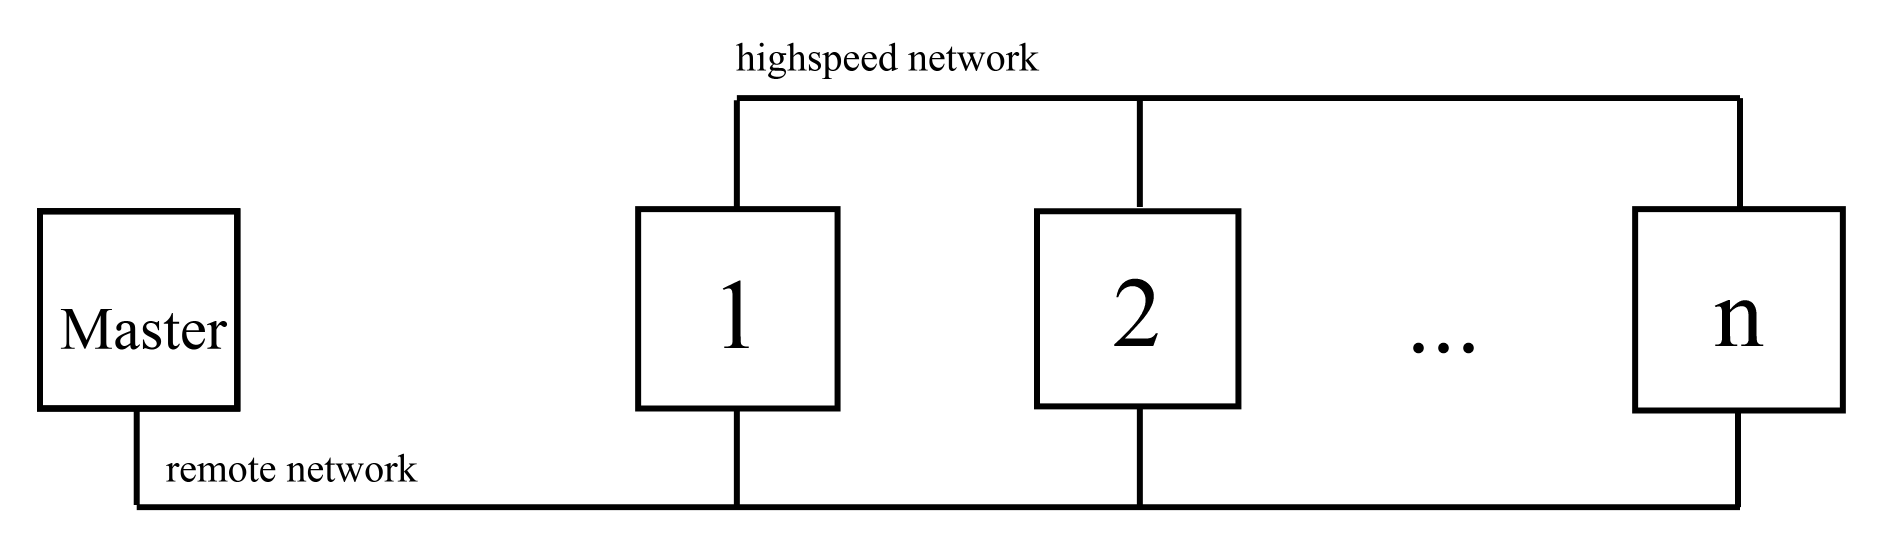
\includegraphics[width=200px]{gfx/cluster_computing.png}
	\caption{cluster computing}
	\label{img:cluster_comp}
\end{figure}
\item grid computing(virtual organisation, geographically distributed and heterogenous))
\end{itemize}
\item distributed inforamtion systems
\begin{itemize}
\item transaction processing systems (database) \\
ACID (atomicity, consistency, isolated, durable)
\item enterprise systems
\end{itemize}
\item Distributed pervasive systems\\
small, wireless, adhoc, no administration\\
home automation, health systems, sensor networks
\end{itemize}

\textbf{Why do we need distributed systems?}\\
\begin{itemize}
\item performance
\item distribution inherent
\item reliability
\item incremental growth (scalability)
\item sharing resources
\end{itemize}

\section{Architectures of distributed Systems}

\begin{itemize}
\item how to split software into components\\
$\Rightarrow$ Softwarearchiticture
\item how to build a system out of the components\\
$\Rightarrow$ Systemarchitecture
\end{itemize}

Middleware can  help to create distribution transparency\\

Architecturestyles:\\
\begin{itemize}
\item Layered architecture\\
$\Rightarrow$ network stack, messages or data flow up and down\\
\begin{itemize}
\item control flow between layers
\item requests down
\item reply up
\end{itemize}
\item Object-based architectures\\
\begin{itemize}
\item interaction between components
\item e.g. remote procedure calls
\item can be client-server system
\end{itemize}
\item data-centered architectures\\
\begin{itemize}
\item data is key element
\item communication over data, distributed database
\item web-systems mostly data-centric
\end{itemize}
\item event-based architecture\\
\begin{itemize}
\item publish-subscribe systems
\begin{figure}[h]
	\centering
	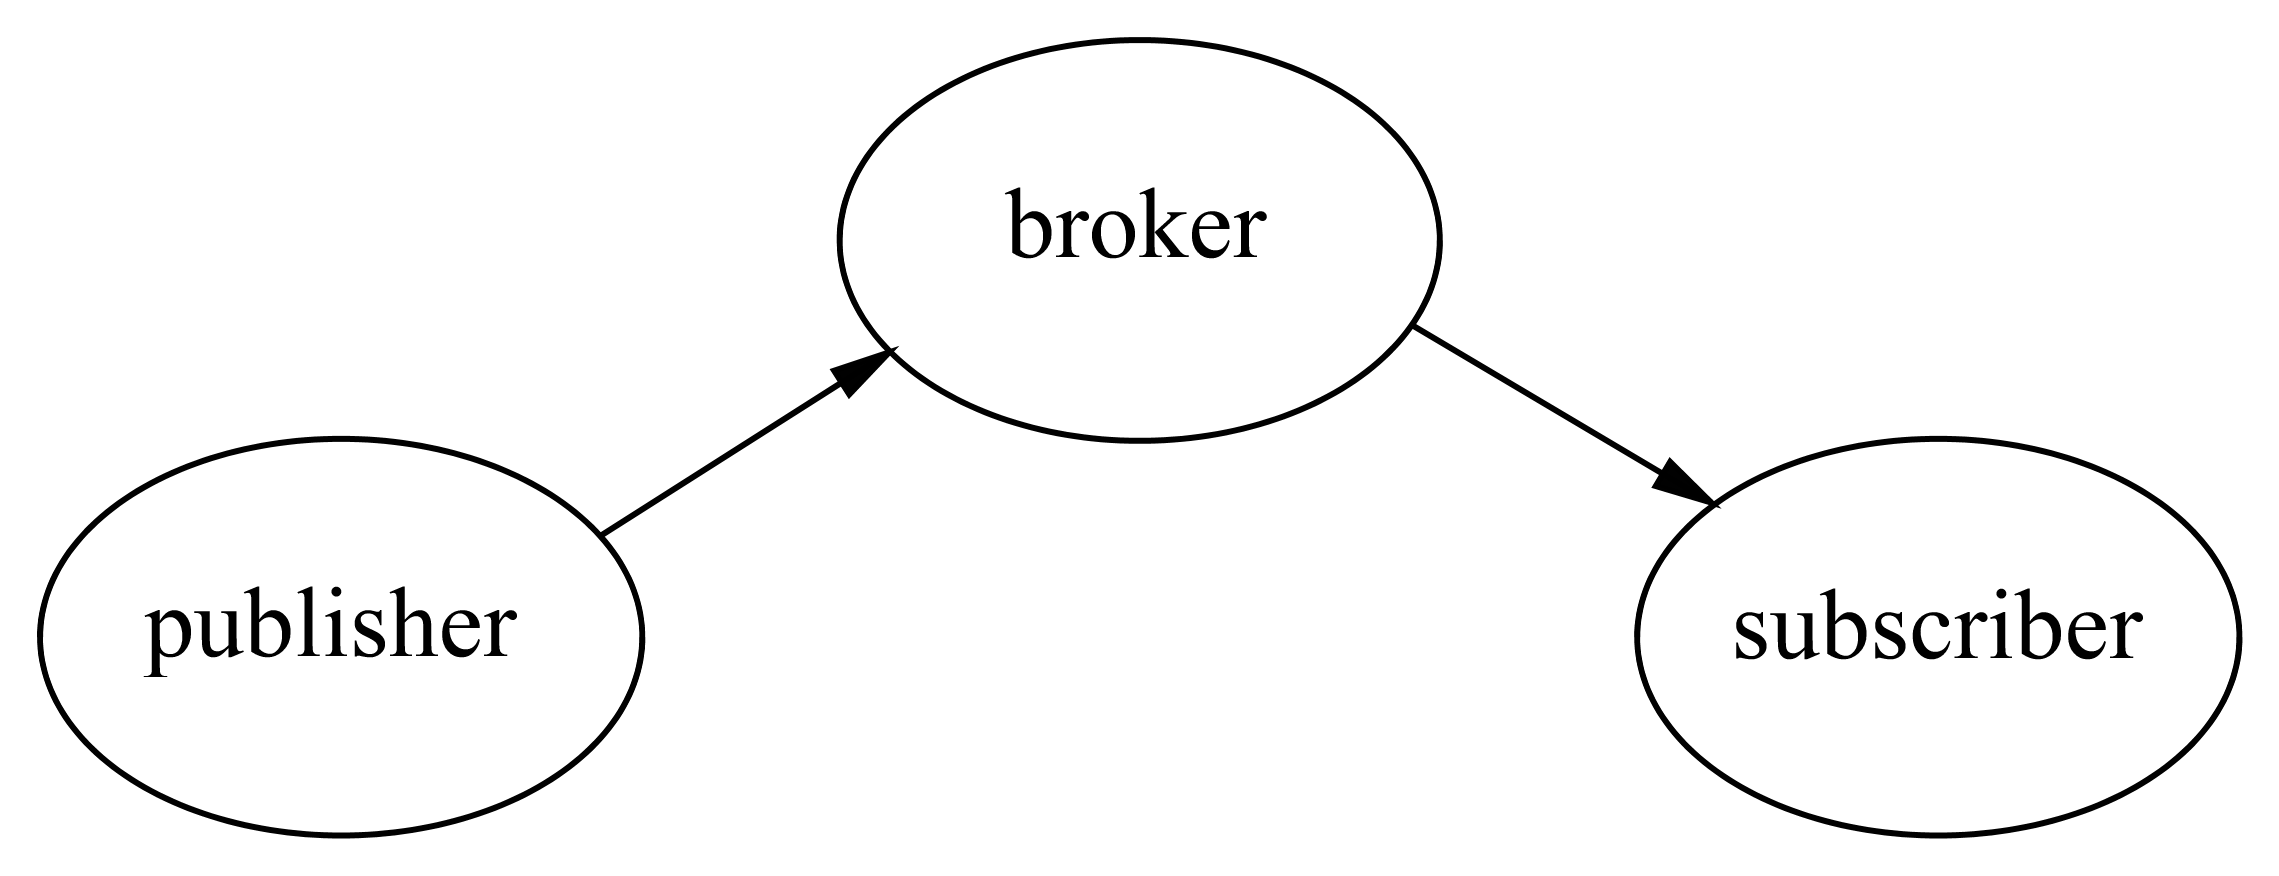
\includegraphics[width=200px]{gfx/pub_sub.png}
	\caption{publish subsribe system}
	\label{img:publish_subscribe}
\end{figure}
\item processes communicates threough events
\item publisher announces events at broker\\
$\Rightarrow$ loose coupling (publisher and subscriber need not to know each other), decoupled in space\\
$\Rightarrow$ scalability better than client-server, parallel processing, caching\\
\end{itemize}
Event-based and data-based can be combined\\
$\Rightarrow$ shared Data space \\
\begin{figure}[h]
	\centering
	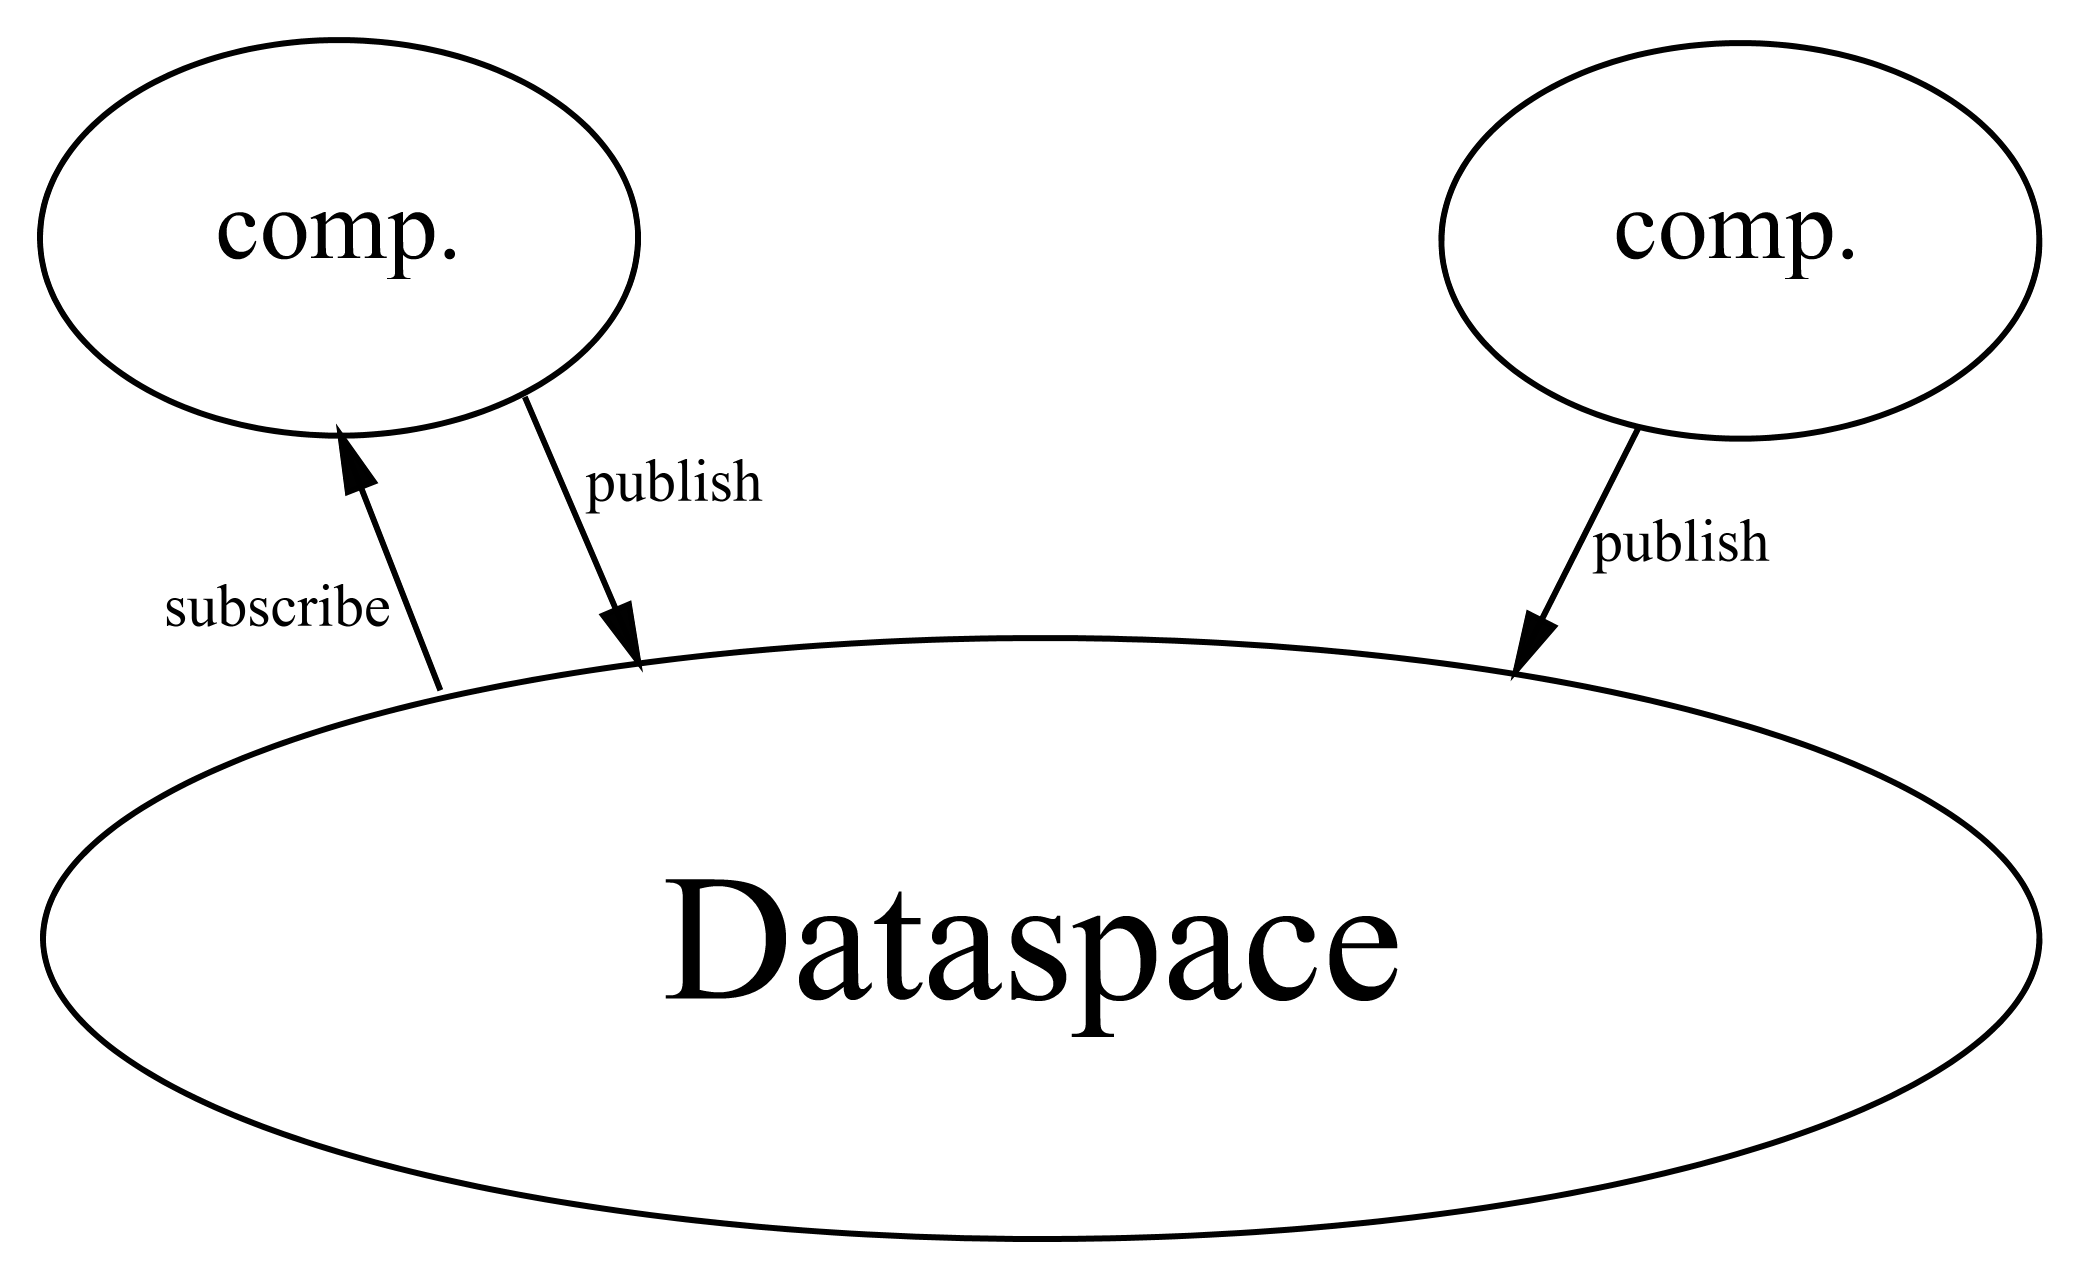
\includegraphics[width=200px]{gfx/shared_data_space.png}
	\caption{shared data space}
	\label{img:shared_data_space}
\end{figure}
\end{itemize}

\subsection{System architectures}
\begin{enumerate}
\item centralized architectures\\
client - server\\
\begin{itemize}
\item[(i)] single point of failure
\item[(ii)] performance (server is bottleneck)\\
\begin{figure}[h]
	\centering
	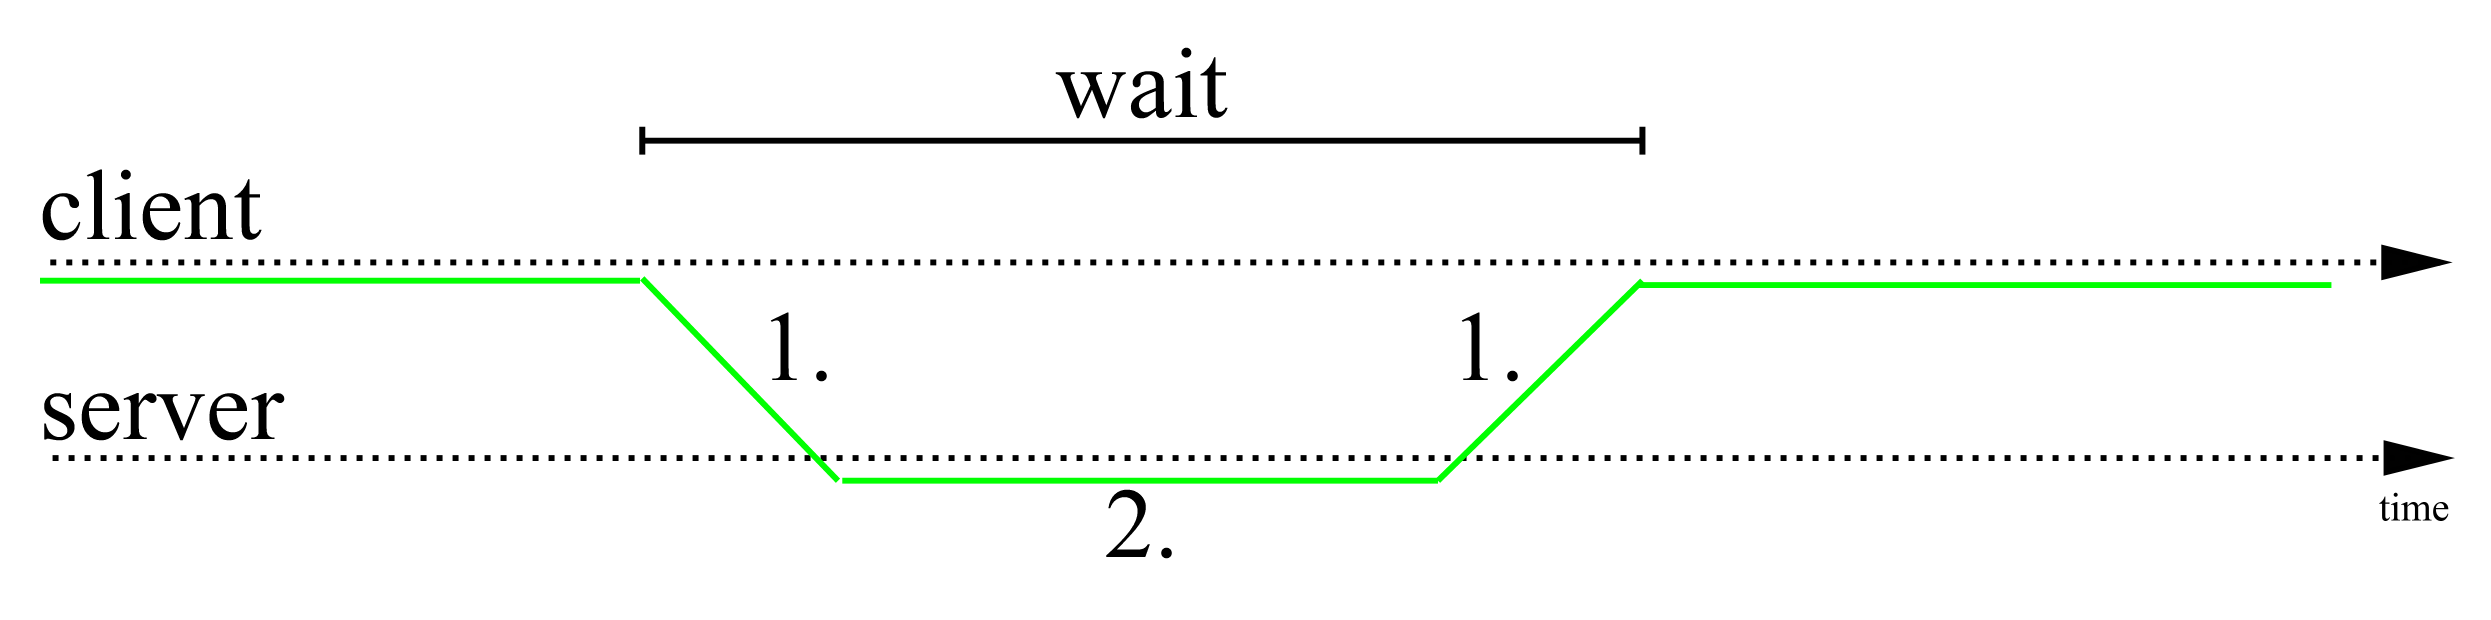
\includegraphics[width=200px]{gfx/cs_simple_wait.png}
	\caption{client server simple waiting situation}
	\label{img:cs_simple_wait}
\end{figure}
\begin{enumerate}
\item communication problems\\
\item server problems\\
\end{enumerate}
can request be repeated without harm?\\
$\Rightarrow$ request is idempotent
\item[(iii)] aplication layering\\
Layers:\begin{itemize}
\item[1.)] User interface
\item[2.)] processing
\item[3.)] data level
\begin{figure}[h]
	\centering
	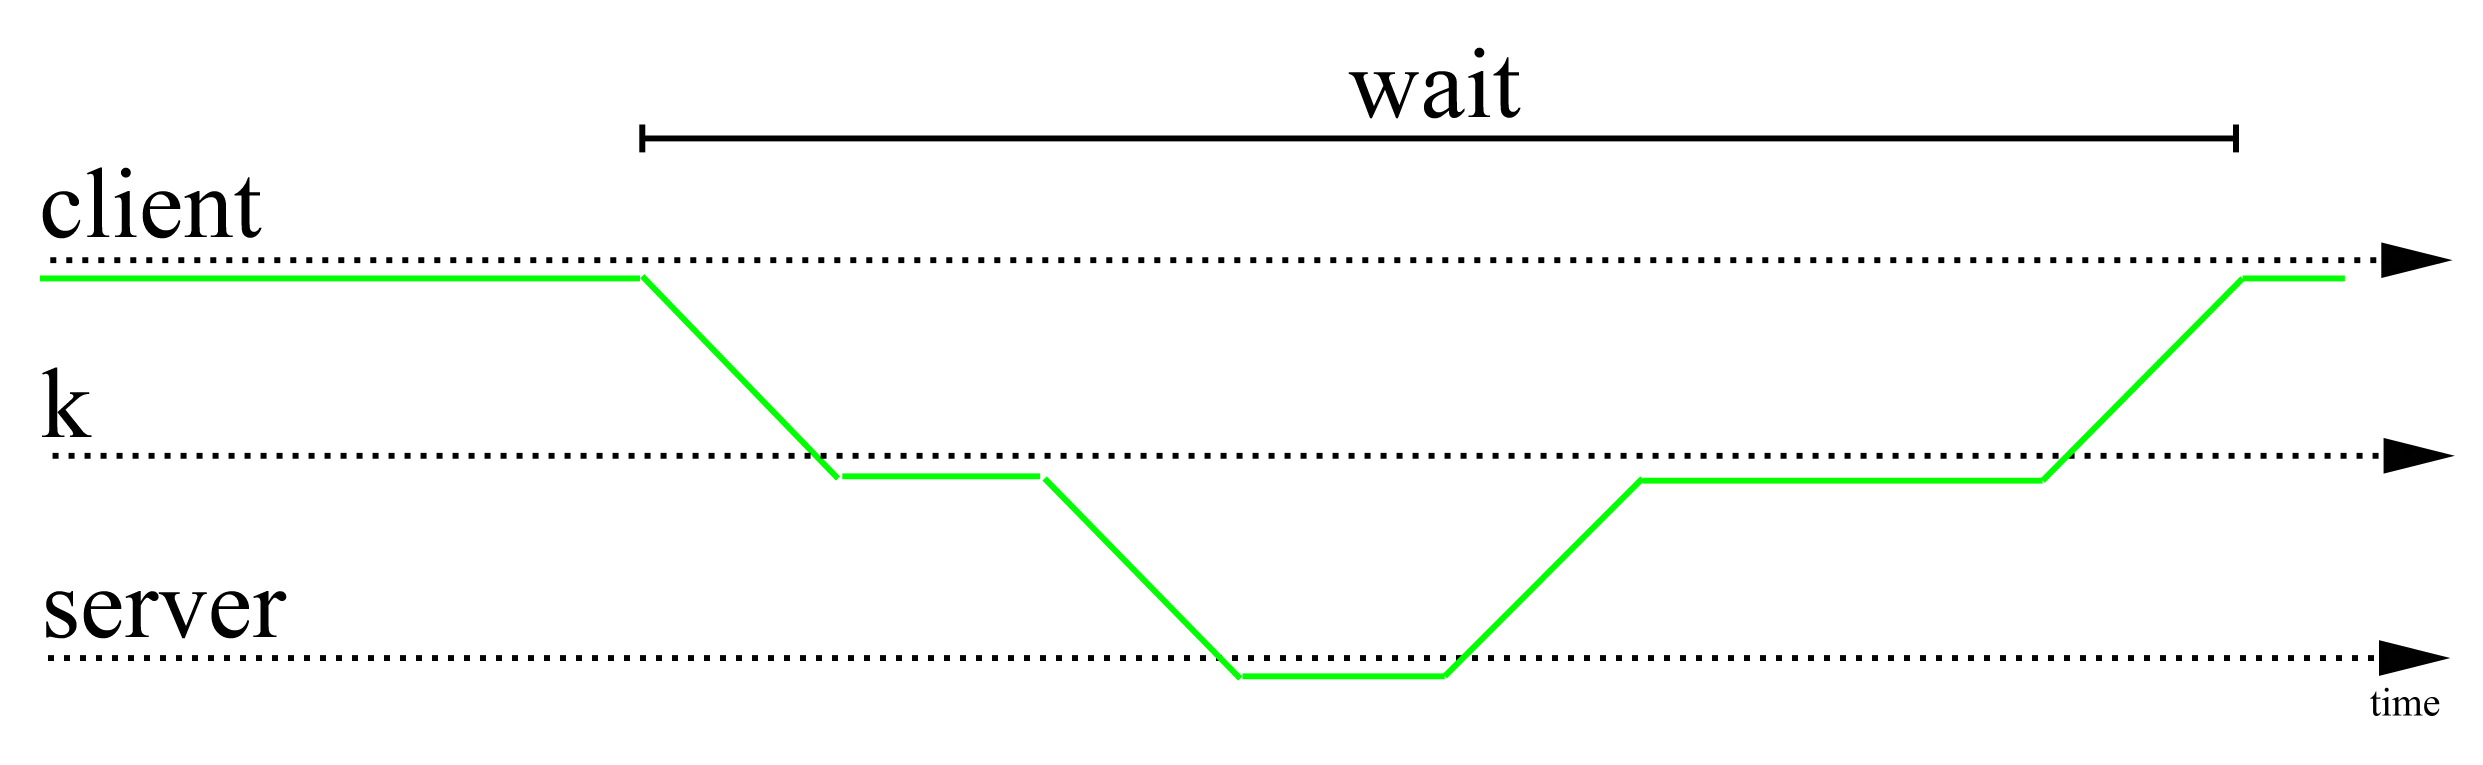
\includegraphics[width=200px]{gfx/cs_app_layer.png}
	\caption{application layer}
	\label{img:cs_app_layer}
\end{figure}
\end{itemize}
$\Rightarrow$ a lot of waiting\\
$\Rightarrow$ does not scale\\
\end{itemize}
\item Decentralized architectures\\
\begin{itemize}
\item vertical distribution (layering)\\
different logic on different machines
\item horizontal distribution \\
replicated client/server operating on different data\\
$\Rightarrow$ overlay-underlay hides physical structure by adding logical structure\\
\end{itemize}

Structured P2P architectures\\
\begin{itemize}
\item most popular technique is distributed hashtables (DHT)\\
\item randomly 128 bit or 160 bit ke for data and nodes. Two or more keys are very unlikely\\
\item Chord system arranges items in a ring 
\item data item k is assigened to node with smallest identifier id $\geq$ k
\end{itemize}
ie item 1 belongs to node 1\\
item 2 belongs to node 2\\
for each item k$_i$ succ(k)=id\\
returns  the name of the node k is assigened to\\
to find data item k the function LOOKUP(k) returns the adress of succ(k) in O(log(N)(later!)\\

membership management\\
join:\\
create SHA1 identifier\\
LOOKUP(id) = succ(id)\\
contact succ(id) and pred(id) to join ring\\

leave:\\
node id informs succ(id) and pred(id) and assigns it's data to succ(id)\\

Content adressable network (CAN)\\
\begin{itemize}
\item d-dimensional cartesian space
\item every node draws random number
\item space is divided among nodes
\item every data draws identifier (coodinates) which assigns a node

\item join\begin{itemize}
\item select random point
\item half the square in which id falls
\item assign item to centers
\end{itemize}
\item leave\begin{itemize}
\item one node takes the rectangle\\
$\Rightarrow$ reassign rectangles periodically
\end{itemize}
\end{itemize}

Unstructured P2P Network\\
\begin{itemize}
\item random graph
\item each node maintains a list of c neighbours
\item partial view or neighbourhood list  with age
\item nodes exchange neighbour information \\active thread\\ select peer\\

PUSH\\
select c/2 youngest entries+myself\\
send to peer\\

PULL\\
receive peer buffer\\
construct new partial view\\
increment age\\

passive thread\\
recieve buffer from peer\\

PULL:\\
select c/2\\
send to peer\\
construct new partial view
increment age\\

\end{itemize}

\end{enumerate}


\section{PeerSim}

\section{Processes}
\begin{tabular}{p{7cm} p{7cm}}
\textbf{processes}			&\textbf{threads}\\
-execution of program			&-several threads share CPU\\
-processor creates virtual processor	&-thread context has little memory information, perhaps mutex lock\\
-for each program everyting is stored in process table	&-threads avoid blocking application (e.g. spreadsheet,computation of dependent cells, intermediate backup)\\
-transparent sharing of resources,(processor, memory) separation&-thread switch is fast\\
-each virtual processor has it's own independent adress space&-user level threads allow parallel computation of program sections\\
-process switch is expensive, (save cpu context, pointers, translation lookaside buffer (TLB), memory management unit (MMU))&I/O or other blocking system calls block all threads, but thread creation/deletion is kernel task = expensive \\
-perhaps even swaps to disk, if memory exhausted& advantages of threads over processes vanishes\\
\end{tabular}

2 possible solutions:\\
\begin{enumerate}
\item scheduler activation, upcall to achieve process switch
\item light-weight processes (LWP)\\
\begin{figure}[h]
	\centering
	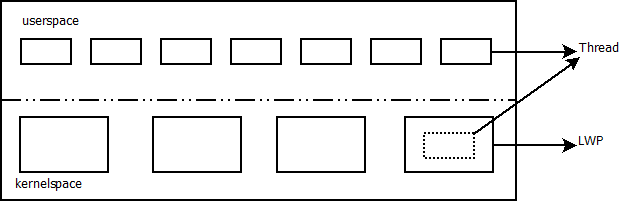
\includegraphics[width=200px]{gfx/thread_lwp.png}
	\caption{light-weight processes can run threads}
	\label{img:lwp_threads}
\end{figure}
user level thread package\\
execute scheduler and run thread of parent\\
may block on systemcall, then other LWP may run\\
triggered from userspace\\
\end{enumerate}
Advantages of LWP and user-level thread package:\\
\begin{enumerate}
\item creation, deletion etc is easy, no kernel intervention
\item blocking syscall does not suspend process if enough LWPs are available
\item applications do not see LWP. They only see user-level threads
\item LWP can run on different processors in multiprocessor systems
\end{enumerate}

Disadvantages:\\
\begin{enumerate}
\item LWP creation as expensive as creation of kernel-level thread
\end{enumerate}

Advantages:\\
- a blocking systemcall blocks only thread, not process
$\Rightarrow$ system call for communication in distributed systems

Multiple threads in clients and servers\\

\textbf{Clients:}\\
\begin{itemize}
\item multiple thread may hide communication delay (distribution transparency)
\item web browser opens several connections to load parts of a document/page
\item web server may be replicated in same or different location\\
$\Rightarrow$ truly parallel access to items and parallel download
\end{itemize}

\textbf{Servers:}\\
\begin{itemize}
\item single threaded, e.g. file server\\
thread serves incoming request, waits for disk, returns file\\
serves next
\item multithreaded\\
dispatcher thread recieves request\\
hands over to worker thread\\
waits for disk etc.\\
dispatcher takes next request
\item finite state machine\\
only one thread\\
examines request, either read from \ldots or from disk\\
during wait stores requests in table\\
serves next request\\
manage control either new request or reply from disk\\
act accordingly\\
process acts as finite state machine that receives messages and acts/changes state
\end{itemize}

\textbf{summary:}\\
\begin{tabular}{l l}
model&characteristics\\
single thread& no parallelism, blocking syscalls\\
multi thread& parallelism, blocking syscalls\\
finite state machine& parallelism, non-blocking syscalls\\
\end{tabular}

\subsection{Virtualisation}
% Bild von Höpster
\begin{figure}[h]
	\centering
	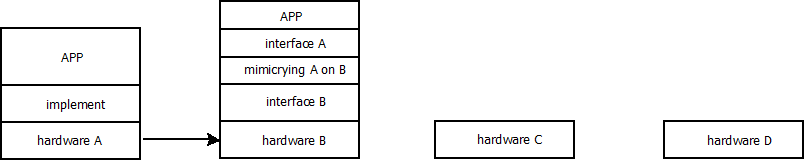
\includegraphics[width=200px]{gfx/virtualisation_1.png}
	\caption{virtualisation}
	\label{img:virtualisation_1}
\end{figure}

V pretends there are more resources then available.\\

Reasons for the need for V.\\
-hardware changes much faster then SW\\
$\Rightarrow$ improves portability\\
-networks consist of different hardware\\
$\Rightarrow$ enables portability of programs for all\\
usage (distributed applications, network protocols)\\

2 Types of Architectures for Virtualisation:\\
\begin{enumerate}
\item Runtime system providing instruction set\\
	\begin{itemize}
	\item interpreted as Java
	\item emulated as for Windows applications on UNIX-platform processes VM
	\end{itemize}
\item Virtualisation shields hardware and offers instruction set of the same or other hardware\\
- can host different OS that run simultaneosly\\
$\Rightarrow$ VMM such as VMware, Xen\\


\end{enumerate}


\subsection{Client-/Serverprocesses}
\textbf{CLients:}\\
%Bild von Tobi !!! :D
\begin{figure}[h]
	\centering
	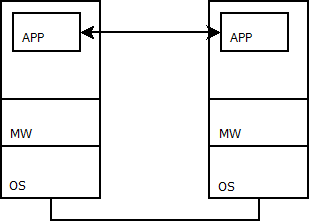
\includegraphics[width=200px]{gfx/clienta.png}
	\caption{app specific communication}
	\label{img:clienta}
\end{figure}
%Mehr Bild!
\begin{figure}[h]
	\centering
	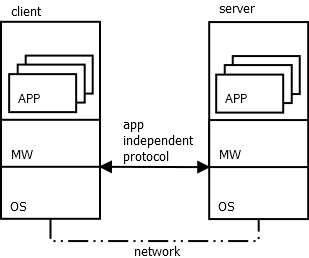
\includegraphics[width=200px]{gfx/clientb.png}
	\caption{machine only communication}
	\label{img:clientb}
\end{figure}

\begin{itemize}
\item b) allows to store data at the server
\item \textbf{thin client} e.g. X-windows
\item thin client should separate application logic from user interaction
\item ooften not implemented $\Rightarrow$ poor performance
\item compression of interaction commands as solution
\item compound documents where user interaction triggers several processing steps on the server. must be implemented (e.g. rotation of picture changes placement in texts)
\end{itemize}

\textbf{Servers:}\\
\begin{itemize}
	\item serves requests on behalf of the client
	\item Types of servers\\
		\begin{itemize}
			\item \textbf{iterative Server} handles requests itself
			\item \textbf{concurrent server} passes requests to worker, e.g. multithreaded server
		\end{itemize}
	\item server listens to port, endpoint to the client; some ports are reserved for special services
\begin{figure}[h]
	\centering
	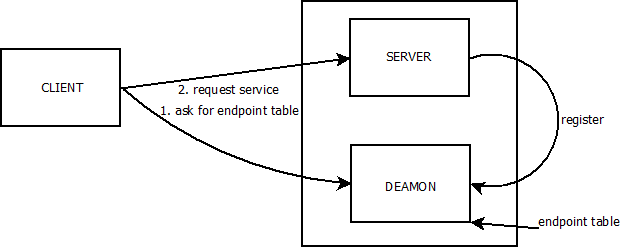
\includegraphics[width=200px]{gfx/server_deamon.png}
	\caption{listener server}
	\label{img:listener}
\end{figure}
	\item superserver listens to several ports, replacinf several (mostly idle) servers
\begin{figure}[h]
	\centering
	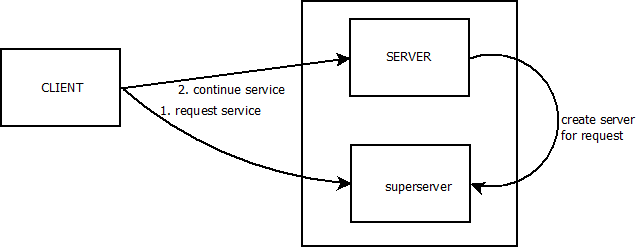
\includegraphics[width=200px]{gfx/superserver.png}
	\caption{superserver}
	\label{img:supserv}
\end{figure}
	\item stateless servers, keeps no information on state of client $\rightarrow$ change state without informing the client, e.g. web server
\begin{figure}[h]
	\centering
	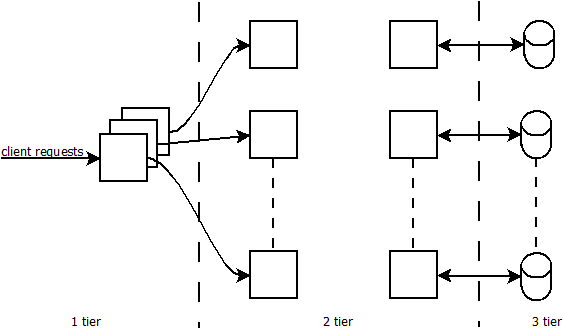
\includegraphics[width=200px]{gfx/server3.png}
	\caption{stateless server}
	\label{img:statel_serv}
\end{figure}
	\item soft state server, maintains client state for limited time, e.g. servers informing about updates
	\item stateful server keeps information about client (file server keeps (client, file) table), often better performance, fault-tolerance poorer
	\item cookies allow to share information for server upon next visit client sends it'S cookies, allows state information for stateless server

\end{itemize}
\textbf{Distributed Servers}\\
\begin{figure}[h]
	\centering
	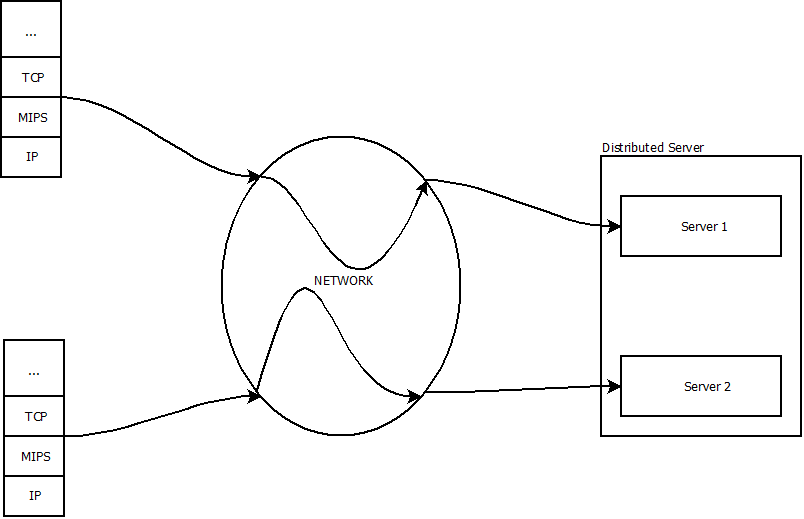
\includegraphics[width=200px]{gfx/distrb_server.png}
	\caption{distributed server}
	\label{img:distrb_serv}
\end{figure}
\begin{itemize}
	\item servers in different locations that have different ip-adresses in DNS under the same name
	\item MIPv6: mobility support for IPv6
	\item mobile node has home network with stable home adress (HoA)
	\item special router is home agent and takes care of traffic to the mobile node
	\item mobile node receives care-of-adress (CoA), never seen by client
	\item route optimisation avoids routing through home agent
\end{itemize}

\subsection{Code Migration}
\begin{itemize}
	\item Code migration on (running) process - Why?
	\item service placement in distributed system $\Rightarrow$ minimize communication cost
	\item load balancing in multiprocessor machine or cluster $\Rightarrow$ performace
	\item (security)

\end{itemize}

\textbf{Models of Migration}
\begin{itemize}
	\item or process model\begin{enumerate}
		\item code segment, instructions
		\item resource segement, references to external resources, ie.e. file, printer, devices
		\item execution segement, execution state process, stack, private data, programm counter

	\end{enumerate}
	\item \textbf{Migration types}\begin{itemize}
		\item weak mobility, transfer code, (1), mabe 3)), which executes from beginning (i.e. java applets)
		\item strong mobility, transfer 1)3), stop executions, transfer, resume
	\end{itemize}
\end{itemize}

%bild

Migrating resource segment 2) is difficult\\
Consider process to resource binding\\
\begin{enumerate}
	\item binding by identifier, URL, ftp-server-name
	\item binding by value, libraries for programming
	\item binding by type, local device, monitor
\end{enumerate}

\textbf{Resource-machine-binding}
\begin{enumerate}
	\item unattached
	\item fastend
	\item fixed
\end{enumerate}

\begin{tabular}{l| l| l| l}
pass tp resource binding&unattached&fastened&fixed\\
\hline
by identifier& MV&GR(or MV)& GR\\
\hline
by value& CP& GR(or CP)& GR\\
\hline
by type& RB&RB(or GR,CP)&RB(or GR)\\
\end{tabular}
MV:move, GR, global reference, CP: copy value, RB: rebind to locally available resource

\section{Communication}
we skip networking $\rightarrow$ Telematik\\

Consider:\\
\begin{itemize}
	\item Remote procedure call
	\item Message-oriented communication
	\item Strem-oriented communication
	\item Multicast communication
\end{itemize}

\subsection{RPC}
%ordinary procedure call, e.g. count = read(fd,buf,nbytes)
Remote procedure call uses stubs to pack parameters in message\\
value parameters\\
$\Rightarrow$ value packed in messages, transfer byte-by-byte$\Rightarrow$ problem can be little endian vs big endian systems\\
reference parameters are: extremely difficult; create array and pass by value; how to handle graps, linked lists\ldots\\






Remote procedure calls\\
\subsection{Asynchronous RPC}
% bild xD

\begin{itemize}
	\item hide communication, communication transparency
\end{itemize}

\subsection{Message oriented communication\\}
\begin{itemize}
	\item avoids synchronous communication which blocks sender\
	Berkely sockets UNIX TCP/IP\\
	server |socket|->|bind|->|listen|->|accept|->|read|<->|write|->|close|\\
	client |socket|------------------->|connect|->|read|<->|write|->|close|\\

\end{itemize}

\subsection{Message-passing-interface (MPI)\\}
\begin{itemize}
	\item standad for communication
	\item communication within group of processes
	\item each group/member has identifier
\end{itemize}

\subsection{Message-queuing-system, Message-oriented-middleware (MoM)}

\begin{itemize}
	\item asynchronous persistent communication\\
	\item store messages
	\item transfer may take minutes, not milliseconds
	\item applications communicate by inserting messages into queues
	\item messages are inserted into local queue
	\item message carries destination adress
	\item queue manager may act as relays, router\\
	%schickes Bild @ Höpster <- INSERT HERE PLX!!!
	\item message broker transform type A into type B, using a set of rules
	\item applications are email, workflow, batch processing, queries accross several databases
\end{itemize}

\subsection{stream oriented communication}
\begin{itemize}
	\item temporal relationship between items important
	\item multimedia data is compressed
	\item QoS is important\\
		\begin{itemize}
			\item bit rate
			\item max delay for session setup
			\item max end-to-end delay
			\item max delay variance (jitter)
			\item max round trip delay\\
				% next pic, tobi
		\end{itemize}
	\item networking solution such as differentiated services
	\item synchronisation of streams
\end{itemize}
\subsection{Multicast communication}
\begin{itemize}
	\item application level multicast uses overlay
	\item tree, unique path between each pair of nodes
	\item mesh, more robust, fault-tolerant
\end{itemize}
\textbf{Example:} Construct overlay tree for chord
\begin{itemize}
	\item node that wants to start multicast generates key 128bit/160bit (nid) randomly
	\item lookup of succ(nid) finds node responsible for key mid\\
		$\Rightarrow$ succ(nid) becomes root of tree
	\item join: lookup (nid) creates lookup message with join request routed from P to succ(nid)
	\item request is forwarded Q (first time forward), Q becomes forwarder\\
		$\Rightarrow$ P child of Q
	\item request is first time forwarded by R, R becomes forwarder\\
		$\Rightarrow$ Q becomes child of R
	\item multicast: lookup(nid) sends message to the root\\
		multicast from root
\end{itemize}
\textbf{Efficiency?}\\
Quality of application level tree\\
\begin{enumerate}
	\item Link stress, number of traversals of same link per packet
	\item stretch, relative delay penalty (RDP)\\
		$\frac{\text{transmission time in overlay}}{\text{transmission time in delay/network}}$
		$\Rightarrow$ minimize aggregated stretch, average RDP over all note pairs
	\item tree cost, minimize aggregated link cost, link cost = cost between end points\\
		$\Rightarrow$ find minimal spanning tree
\end{enumerate}
\subsection{Gossip-based-communication}
\begin{itemize}
	\item epidemic behaviour
	\item a node does not have new data (susceptible), it has the data (infected) or is unwilling to spread (removed)\\
	Anti-entropy-model\\
	P chooses randomly Q\\
	\begin{enumerate}
		\item P pushes its data to Q
		\item P pulls Q's data
		\item P and Q exchange data
	\end{enumerate}
	\item if many nodes are infected probabiltry for selecting susceptible node  is low\\
	$\Rightarrow$ low probability of data dissemination\\
	\item pull works when many nodes are infected. Susceptible node determines spread. They have a high probability to contact infected nodes
	\item if only one node is infected push/pull is best
	\item Round is period in which each node at least once selects a neighbor\\
		number of rounds needed to spread  $\approx \mathcal{O}(\log(N)), N$ is number of nodes\\
\end{itemize}
\textbf{Rumor spreading, gossiping}:\\
%bild
function of nodes that never obtain data: $s=e^{-(k+1)(1-s)}$\\
e.g. $k=4, ln(s) = 4,97$\\
$\Rightarrow s = 0,007$\\
less than $0,7$ remain without data\\
removing data is difficult : delete message is send via gossiping

\end{document}
